
\section{MODELING AND SIMULATING BODY BIASING INJECTION}
%\begin{frame}
%    \frametitle{Simulation models}
%    \begin{itemize}
%        \setlength\itemsep{1em}
%        \item What is interesting in developing simulation models?
%        \vspace{0.2cm}
%        \begin{itemize}
%            \setlength\itemsep{0.9em}
%            \item No dedicated CAD tools;
%            \item Very difficult to physically observe the IC from the inside.
%        \end{itemize}
%        \item Therefore → mixed approach simulation/experiments.
%    \end{itemize}
%\end{frame}

\begin{frame}{Why modeling and simulating BBI?}
    \Large
    Observe the signals inside the IC:
    \begin{itemize}
        \setlength\itemsep{1em}
        \normalsize
        \item Embedded sensors → costly and long to implement
        \item Will be disturbed by the voltage pulses
    \end{itemize}
    \vspace{10mm}
    \centering
    \LARGE Therefore: simulation → conclusions → verification
\end{frame}

\begin{frame}{Simulation models}
    \begin{textblock*}{5cm}(5mm, 20mm)
        \onslide<1-6>{\includegraphics[width=\textwidth]{psuNetworkNew.png}}
    \end{textblock*}

    \begin{textblock*}{2cm}(15mm, 38mm)
        \onslide<2-6>{\begin{tikzpicture}
            \draw[-Stealth, blue, thick] (0, 0) -- (0.5, -0.5);
        \end{tikzpicture}}
    \end{textblock*}

    \begin{textblock*}{5cm}(8mm, 45mm)
        \onslide<2-6>{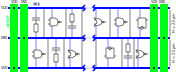
\includegraphics[width=0.8\textwidth]{std_cell_segment_principle.pdf}}
    \end{textblock*}

    \begin{textblock*}{2cm}(15mm, 63mm)
        \onslide<3-6>{\begin{tikzpicture}
            \draw[-Stealth, blue, thick] (0, 0) -- (0.0, -0.5);
        \end{tikzpicture}}
    \end{textblock*}

    \begin{textblock*}{3cm}(11mm, 68mm)
        \onslide<3-6>{\includegraphics[width=0.8\textwidth]{DUAL.pdf}}
    \end{textblock*}

    \begin{textblock*}{3cm}(13mm, 85.5mm)
        \onslide<3-6>{\small DUAL-WELL}
    \end{textblock*}

    \begin{textblock*}{3cm}(35mm, 68mm)
        \onslide<3-6>{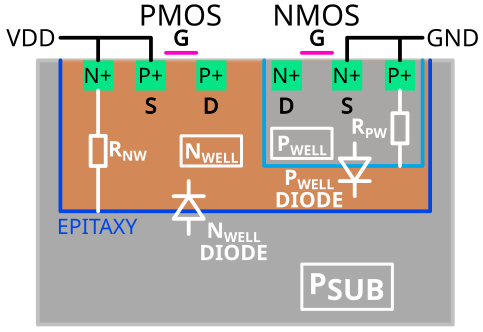
\includegraphics[width=0.8\textwidth]{TRIPLE.pdf}}
    \end{textblock*}

    \begin{textblock*}{3cm}(36.5mm, 85.5mm)
        \onslide<3-6>{\small TRIPLE-WELL}
    \end{textblock*}

    \begin{textblock*}{2cm}(60mm, 63.5mm)
        \onslide<4-6>{\begin{tikzpicture}
            \draw[-Stealth, blue, thick] (0, 0) -- (0.5, 1.2);
        \end{tikzpicture}}
    \end{textblock*}

    \begin{textblock*}{2cm}(67mm, 41mm)
        \onslide<4-6>{
\begin{tikzpicture}
            \draw[decorate, decoration={brace}, blue, thick] (0, 0) -- (0.0, 4.5);
        \end{tikzpicture}}
    \end{textblock*}

    \begin{textblock*}{4.7cm}(70mm, 42.5mm)
        \onslide<4-6>{\includegraphics[width=0.8\textwidth]{dualWell_no_7c_Eevee.png}}
    \end{textblock*}

    \begin{textblock*}{4.7cm}(109.5mm, 41.5mm)
        \onslide<4-6>{
\begin{tikzpicture}
            \draw[-, black, line width=0.4mm] (0, 0) -- (0.0, 4.5);
        \end{tikzpicture}}
    \end{textblock*}

    \begin{textblock*}{4.7cm}(109.5mm, 32mm)
        \onslide<5-6>{\begin{tikzpicture}
            \draw[-Stealth, blue, line width=0.4mm] (0, 0) -- (0.5, 0.72);
        \end{tikzpicture}}
    \end{textblock*}

    \begin{textblock*}{2cm}(68mm, 40mm)
        \onslide<5-6>{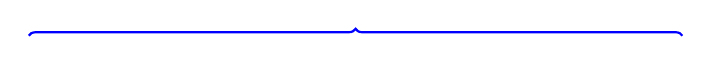
\begin{tikzpicture}
                \draw[decorate, decoration={brace}, blue, thick] (0, 0) -- (8.3, 0.0);
        \end{tikzpicture}}
    \end{textblock*}

    \begin{textblock*}{4.7cm}(112mm, 42.5mm)
        \onslide<4-6>{\includegraphics[width=0.8\textwidth]{tripleWell_no_7c_Eevee.png}}
    \end{textblock*}

%    \begin{textblock*}{2cm}(125mm, 55mm)
%        \onslide<5-6>{\begin{tikzpicture}
%%            \draw[-Stealth, blue, thick] (0, 0) -| (2.0, 0.6) -- (0.5, 2.5);
%            \draw[-Stealth, blue, thick] (0, 0) -| (1.7, 1.7);
%        \end{tikzpicture}}
%    \end{textblock*}

    \begin{textblock*}{5cm}(110mm, 5mm)
        \onslide<5-6>{\includegraphics[width=0.8\textwidth]{resultingSimulated_ic.png}}
    \end{textblock*}

    \begin{textblock*}{1.5cm}(73mm, 12mm)
        \onslide<6-6>{
\includegraphics[width=1.0\textwidth]{generatorModel.pdf}}
    \end{textblock*}

    \begin{textblock*}{1.5cm}(72mm, 11mm)
        \onslide<6-6>{
        
\begin{tikzpicture}
            \draw[blue, line width=0.5mm] (0, 0) rectangle ++(1.7, 2.3);
        \end{tikzpicture}}
    \end{textblock*}

%    \begin{textblock*}{2cm}(60mm, 30mm)
%        \onslide<6-6>{\begin{tikzpicture}
%            \draw[-Stealth, blue, thick] (0, 0) -- (1.0, 0.0);
%        \end{tikzpicture}}
%    \end{textblock*}

    \begin{textblock*}{2cm}(95mm, 22.5mm)
        \onslide<6-6>{\begin{tikzpicture}
            \draw[-Stealth, blue, thick] (0, 0) -- (1.0, 0.0);
        \end{tikzpicture}}
    \end{textblock*}

%    \begin{textblock*}{8cm}(4cm, 1.75cm)
%        \centering
%        \onslide<7->{\includegraphics[width=1.0\textwidth]{resultingSimulated_ic.png}}
%    \end{textblock*}

\end{frame}
